\chapter{系统发生树与分子钟}\label{ch:b2:phylogenetic-trees}

1965 年，两位化学家埃米尔·祖克坎德尔与鲍林
比较了少数几种脊椎动物血红蛋白的氨基酸序列，
并注意到一个解剖学家无论如何也看不到的现象：
两个物种之间的差异数，与其祖先分开的时间成正比，
而该时间可由化石读出。
分子会记录时间。十年之内，卡尔·乌斯利用了一个基因，
即小核糖体亚基的 RNA，绘制出了所有生命的树，
并在其中发现了第三域——古菌，在
显微镜下它与细菌无从区分。本章讨论的是
如何由相似性重建历史：树意味着什么，
一棵树如何由性状与距离构建，序列如何
被用于计时，以及读树者须知的陷阱——趋同、速率不均、
饱和与长枝。

\section{读树}

\begin{definition}[系统发生、演化支、同源性]\label{def:b2:phylogenetic-trees:tree}
\index{系统发生}\index{演化支}\index{单系群}\index{并系群}\index{多系群}\index{同源性}\index{同功性}\index{共有衍征}
\emph{系统发生}是一棵树，其末端为所比较的物种（或基因、
或个体），其内部节点为它们的共同祖先，
其根为一切祖先中最古老者。其
分支次序本身即承载历史：节点可以任意旋转，
只有嵌套关系有意义。\emph{演化支}或
\emph{单系群}是指包含某祖先及其\emph{全部}后代的类群
（鸟类；哺乳动物；鸟类与鳄类合在一起）；
\emph{并系群}是指某祖先去掉部分后代之后的类群
（“爬行动物”去掉鸟类，“鱼类”去掉四足动物，
“\omterm{def:b2:unicellular-diversity:prokaryote}{原核生物}”）；\emph{多系群}则将来自不同祖先的后代
凭各自独立演化而来的相似性归为一组
（“恒温动物”）。两个物种共有的性状
若因其祖先已具有而共有，则为\emph{同源性}（蝙蝠翼
与鲸鱼鳍肢的骨骼）；若二者各自独立演化而来，
则为\emph{同功性}或\emph{同塑性}（蝙蝠与鸟类的翅膀，
以及脊椎动物与章鱼的照相眼）。只有同源性
才记录历史，其中只有
一个类群共有的\emph{衍生的}状态——即其
\emph{共有衍征}（亨尼希的用语）——才能界定演化支：羽毛界定鸟类，
而祖先状态“无羽毛”则不界定任何类群。
\end{definition}

\begin{omfigure}
\begin{tikzpicture}[every node/.style={font=\scriptsize}, >=stealth, line width=0.8pt]
  \coordinate (root) at (0,0);
  \coordinate (n1) at (1.2,0.9); \coordinate (n2) at (2.4,1.6); \coordinate (n3) at (3.6,2.3);
  \draw (root) -- (1.4,-1.3) node[right] {哺乳动物};
  \draw (root) -- (n1);
  \draw (n1) -- (4.8,-0.1) node[right] {龟类};
  \draw (n1) -- (n2);
  \draw (n2) -- (4.8,0.9) node[right] {蜥蜴、蛇};
  \draw (n2) -- (n3);
  \draw (n3) -- (4.8,1.9) node[right] {鳄类};
  \draw (n3) -- (4.8,3.0) node[right] {鸟类};
  \fill (root) circle (1.6pt); \fill (n1) circle (1.6pt); \fill (n2) circle (1.6pt); \fill (n3) circle (1.6pt);
  \node[left] at (root) {羊膜动物};
  % groups
  \draw[omThm, thick, rounded corners=6pt] (3.1,1.55) rectangle (6.9,3.4);
  \node[omThm, anchor=south west] at (3.1,3.4) {主龙类：单系};
  \draw[omExo!80!black, thick, dashed, rounded corners=6pt] (2.2,-0.5) -- (2.2,2.2) -- (7.1,2.2) -- (7.1,-0.5) -- cycle;
  \node[omExo!80!black, anchor=north east] at (7.1,-0.55) {“爬行动物”去掉鸟类：并系};
  \node[anchor=west, align=left, text width=4.2cm] at (7.9,1.3) {共有衍征：\\ $\bullet$ 羊膜卵（全部）\\ $\bullet$ 颅骨上的眶前孔（主龙类）\\ $\bullet$ 羽毛（鸟类）};
\end{tikzpicture}

{\small 读树。鸟类嵌套在爬行动物之中：鳄类
与鸟类的亲缘关系比与蜥蜴更近。所谓“爬行动物”
是指去掉一支后代的祖先，即一个\omterm{def:b2:phylogenetic-trees:tree}{并系
群}，而非\omterm{def:b2:phylogenetic-trees:tree}{演化支}。}
\end{omfigure}

\begin{omfigure}
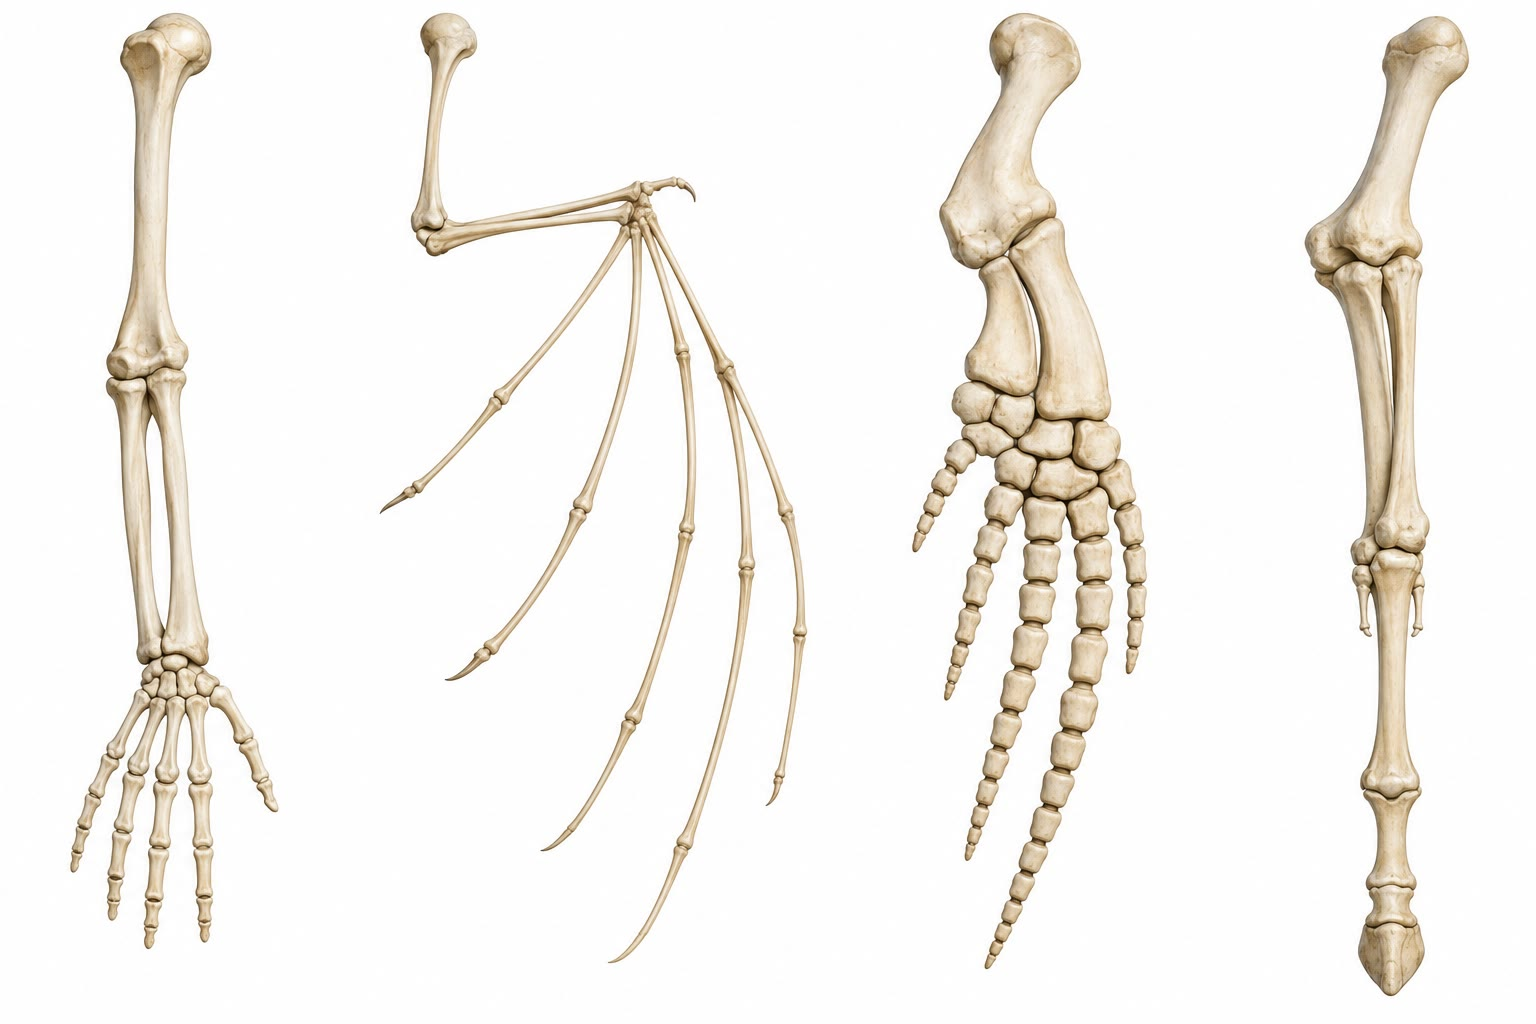
\includegraphics[width=0.44\linewidth]{images/book4/ai/b4-24-homologous-forelimbs.jpg}\hspace{0.04\linewidth}
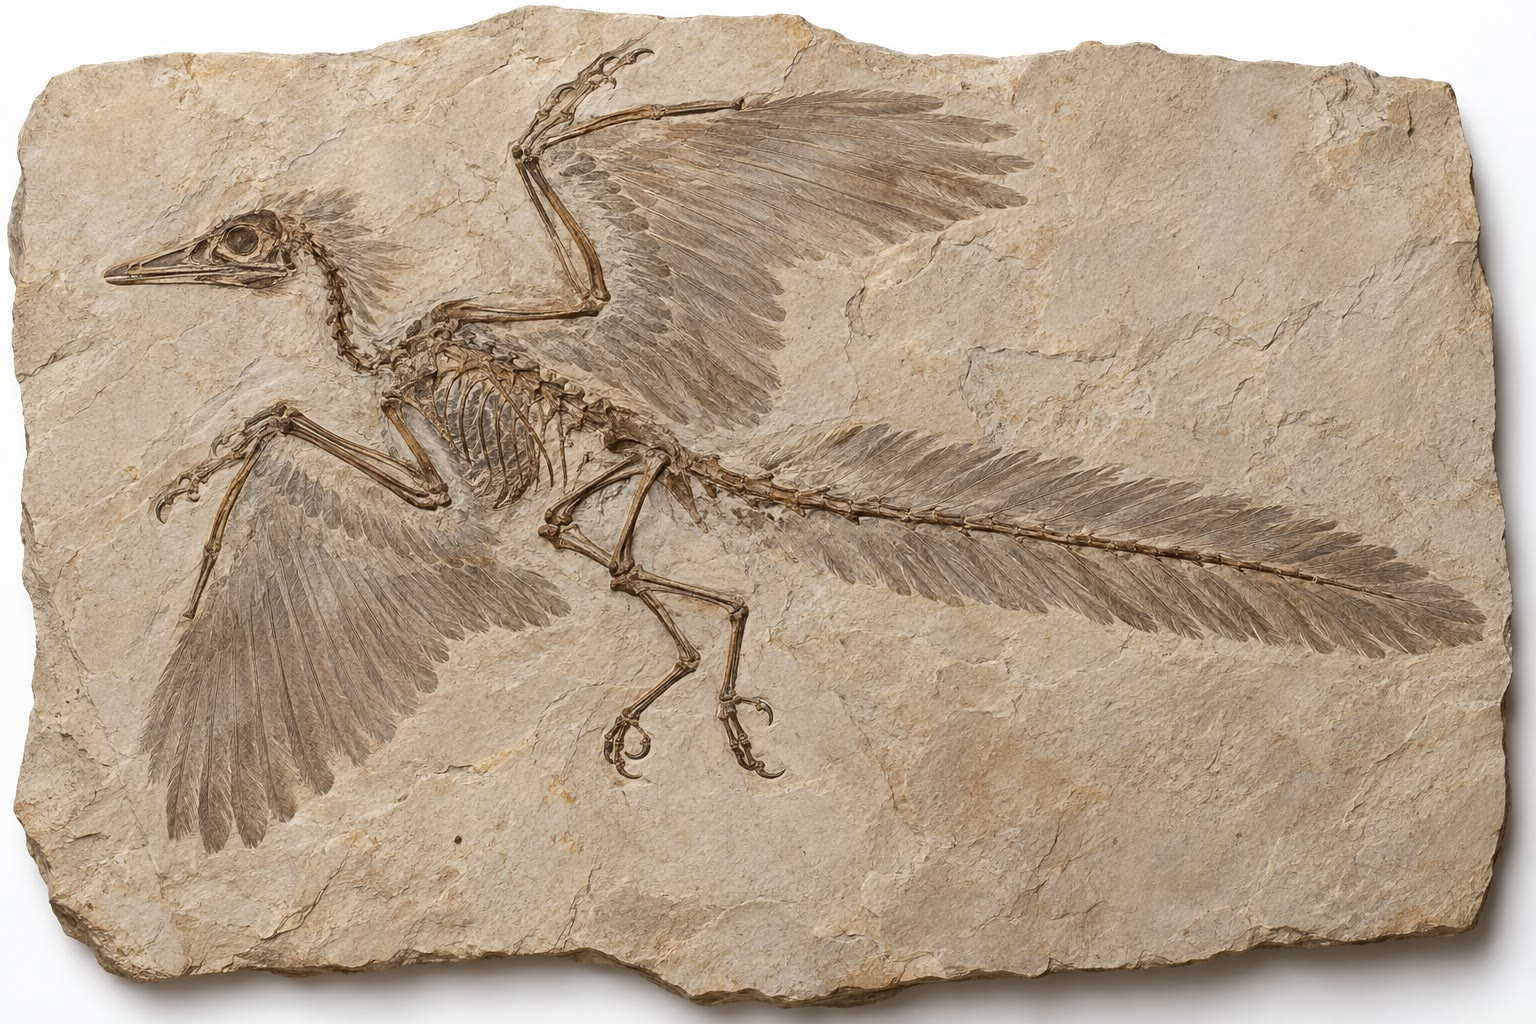
\includegraphics[width=0.44\linewidth]{images/book4/ai/b4-24-archaeopteryx.jpg}

{\small \omterm{def:b2:phylogenetic-trees:tree}{同源性}及其记录。左：同样的骨骼——肱骨、
桡骨与尺骨、腕、五指——见于手臂、翅膀、
鳍状肢和腿中。右：\emph{Archaeopteryx}，带有牙齿、
爪状指与小型恐龙的长骨质尾，同时具有
鸟类的羽毛。}
\end{omfigure}

\section{由性状构建树}

\begin{method}[简约法]\label{meth:b2:phylogenetic-trees:parsimony}
\index{简约法}\index{外群}\index{自展法}
为各分类单元的性状（形态学状态或比对后的序列位点）
逐一赋值。对每一种可能的树，统计解释这些数据
在该树上所需的最少性状变化次数，
其中变化数最少者为最简约树。用一个
\emph{\omterm{meth:b2:phylogenetic-trees:parsimony}{外群}}为树定根，\omterm{meth:b2:phylogenetic-trees:parsimony}{外群}即已知位于所研究类群之外的分类单元。
由于 $n$ 个分类单元的无根树数目为 $1\cdot 3\cdot
5\cdots(2n - 5)$——四个分类单元时为三棵，十个时为 $2\times 10^{6}$ 棵，
二十个时为 $10^{20}$ 棵——故穷举搜索只适用于小
规模，更大时则用启发式搜索。可信度以
\emph{\omterm{meth:b2:phylogenetic-trees:parsimony}{自展法}}度量：有放回地对性状重抽样一千次，
每次重建树，记录每个\omterm{def:b2:phylogenetic-trees:tree}{演化支}重现的频率；
若某\omterm{def:b2:phylogenetic-trees:tree}{演化支}出现于\qty{95}{\%}的重抽样中，
则支持充分；出现于一半者则不然。
\end{method}

\begin{example}[四个分类单元，五个位点]\label{ex:b2:phylogenetic-trees:parsimony}
序列 $A = \mathrm{AAGCT}$、$B = \mathrm{AAGCC}$、$C =
\mathrm{GGACT}$、$D = \mathrm{GGATC}$。在树 $((A,B),(C,D))$ 上，
位点 1、2、3 各变化一次（均在内部分支上），位点 4
变化一次（$\mathrm{C}\to\mathrm{T}$，发生于 $D$），位点 5 变化两次
（$\mathrm{T}\to\mathrm{C}$，发生于 $B$ 与 $D$）：共六步。在
树 $((A,C),(B,D))$ 上，位点 1--3 各需两次变化，位点 4 和 5
各一次：共八步。在 $((A,D),(B,C))$ 上：共九步。第一棵树
最简约，少两步；支持它的三个位点即为其
\omterm{def:b2:phylogenetic-trees:tree}{共有衍征}，而位点 5 在该树上为同塑性——同一变化
发生两次，这在每个真实数据集中都屡见不鲜。
\end{example}

\begin{omfigure}
\begin{tikzpicture}[every node/.style={font=\scriptsize}, line width=0.8pt]
  \foreach \x/\a/\b/\c/\d/\steps/\lab in {0/A/B/C/D/6/{$((A,B),(C,D))$——6 步}, 4.6/A/C/B/D/8/{$((A,C),(B,D))$——8 步}, 9.2/A/D/B/C/9/{$((A,D),(B,C))$——9 步}} {
    \begin{scope}[xshift=\x cm]
      \draw (0,1.6) node[left] {\a} -- (0.8,1.1) -- (0,0.6) node[left] {\b};
      \draw (0.8,1.1) -- (2.0,1.1);
      \draw (2.8,1.6) node[right] {\c} -- (2.0,1.1) -- (2.8,0.6) node[right] {\d};
      \node[anchor=north] at (1.4,0.2) {\lab};
    \end{scope}
  }
  \node[anchor=north] at (5.9,-0.6) {\begin{tabular}{l@{\ }ccccc} 位点 & 1 & 2 & 3 & 4 & 5 \\ \hline $A$ & A & A & G & C & T \\ $B$ & A & A & G & C & C \\ $C$ & G & G & A & C & T \\ $D$ & G & G & A & T & C \end{tabular}};
\end{tikzpicture}

{\small 四个分类单元的三棵无根树，依其下方的五位点
比对计分。位点 1--3 在第一棵树上各变化一次，
在另外两棵上各变化两次；位点 4 仅在一个分类单元中变化，
无法作出判断，而位点 5 将 $A$ 与 $C$ 归为一组，
因而支持第三棵树、反对其余两棵。}
\end{omfigure}

\section{由距离建树}

\begin{method}[按距离聚类：UPGMA]\label{meth:b2:phylogenetic-trees:upgma}
\index{UPGMA}\index{邻接法}\index{距离矩阵}
由 $n$ 个分类单元两两之间的距离（每位点的差异数，
按下文校正），将距离最近的一对合并为一个类，
该类置于高度为其距离一半的节点上；以该类替代这一对，
新类到其他每个分类单元的距离取其成员距离的平均值；
如此重复，直至只剩一个类。所得结果
为有根树，所有末端位于同一高度——这一方法假定每一分支上的
变化速率恒定，即分子钟。谱系之间速率不同时，该方法会
把演化较快的谱系归为一组，不论其历史如何；
\emph{\omterm{meth:b2:phylogenetic-trees:upgma}{邻接法}}，
每一步选择合并后能使整棵树总长缩短最多的一对，
它不假定分子钟，是处理
大型数据集的标准快速方法。
\end{method}

\begin{example}[UPGMA]\label{ex:b2:phylogenetic-trees:upgma}
距离（以每百位点的差异数计）：$AB = 4$，$AC = 8$，
$AD = 10$，$BC = 8$，$BD = 10$，$CD = 6$。将 $A$ 与 $B$ 在高度 2 处合并；
随后得 $d(AB, C) = 8$，$d(AB, D) = 10$，$d(C,D) = 6$：将 $C$ 与 $D$ 在
高度 3 处合并；最后 $d(AB, CD) = (8 + 10 + 8 + 10)/4 = 9$，将两个类在
高度 $4.5$ 处合并。所得树为 $((A,B),(C,D))$，若
速率为每位点每年 $10^{-9}$ 次替换，则根的年龄为
$0.045/10^{-9} = 45$，即 4500 万年。
\end{example}

\begin{omfigure}
\begin{tikzpicture}[every node/.style={font=\scriptsize}, line width=0.8pt, x=1.1cm]
  \draw[->] (0,-0.4) -- (5,-0.4); \foreach \h in {0,1,2,3,4} \draw (\h,-0.5) -- (\h,-0.3) node[below=4pt] {\h};
  \node[anchor=north] at (2.5,-0.9) {节点高度（每百位点的差异数）};
  % A,B join at 2, C,D at 3, root at 4.5 ; draw as rooted tree, root on the right
  \draw (0,3.0) node[left] {$A$} -- (2,3.0) -- (2,2.4) -- (0,2.4) node[left] {$B$};
  \draw (0,1.2) node[left] {$C$} -- (3,1.2) -- (3,0.4) -- (0,0.4) node[left] {$D$};
  \draw (2,2.7) -- (4.5,2.7) -- (4.5,0.8) -- (3,0.8);
  \fill (2,2.7) circle (1.5pt); \fill (3,0.8) circle (1.5pt); \fill (4.5,1.75) circle (1.5pt);
  \node[anchor=west] at (4.6,1.75) {根，4.5};
  \node[anchor=south west] at (2.05,3.05) {2};
  \node[anchor=south west] at (3.05,1.25) {3};
  \node[anchor=west, align=left] at (6.2,2.4) {\begin{tabular}{c|ccc} & $B$ & $C$ & $D$ \\ \hline $A$ & 4 & 8 & 10 \\ $B$ & & 8 & 10 \\ $C$ & & & 6 \end{tabular}};
  \node[anchor=west, align=left] at (6.2,0.7) {合并 $AB$ 后：\\ $d(AB,C) = 8$，$d(AB,D) = 10$\\ 合并 $CD$ 后：$d(AB,CD) = 9$};
\end{tikzpicture}

{\small 四个分类单元上的 \omterm{meth:b2:phylogenetic-trees:upgma}{UPGMA}。每个节点位于所合并两类之间
距离的一半处；所有末端位于高度零，
正如分子钟所要求的。}
\end{omfigure}

\section{分子钟}

\begin{theorem}[替换作为泊松过程，以及多重命中的校正]\label{thm:b2:phylogenetic-trees:clock}
\index{分子钟}\index{朱克斯–康托尔校正}\index{饱和}
若某位点的替换以每年 $k$ 的恒定速率发生，
且各位点相互独立，则沿一条谱系在时间 $t$ 内积累的替换数
服从均值为 $kt$ 的泊松分布，而
两谱系在 $t$ 年前\omterm{def:b2:cell-differentiation:differentiation}{分化}，其间的期望替换数为
\[
d = 2kt
\]
每位点的替换数——即\emph{分子钟}。观察到的
发生差异的位点比例 $p$ 小于 $d$，因为一个
位点若被替换两次，可能回到原碱基，或偶然相同；
设四种碱基以相同速率变化，则
\[
p = \tfrac{3}{4}\bigl(1 - e^{-4d/3}\bigr), \qquad
d = -\tfrac{3}{4}\ln\bigl(1 - \tfrac{4}{3}p\bigr),
\]
\emph{朱克斯–康托尔}校正。随着 $d$ 增大，$p$ 趋于饱和，
极限为 $3/4$——两条随机序列在四分之一的位点上一致
——超过 $p \approx 0.5$ 后，校正会放大每一个
抽样误差：一个已变化到这种程度的基因，已不再
能准确计时。慢速基因（核糖体 RNA、组蛋白）用于推算深层
分支，快速基因（线粒体 DNA、内含子）用于推算近期分支。
\end{theorem}
\begin{proof}
设 $q(t)$ 为一位点在时间 $t$ 之后仍保留
其原有碱基的概率。该位点以速率 $k$ 失去原碱基，
并从其他三种碱基中任一种回复，速率为 $k/3$：
$\mathrm{d}q/\mathrm{d}t = -kq + \tfrac{k}{3}(1 - q) = \tfrac{k}{3} -
\tfrac{4k}{3}q$，其在 $q(0) = 1$ 下的解为 $q = \tfrac14 +
\tfrac34 e^{-4kt/3}$。两条谱系相隔总时间 $2t$——
由对称性，这等同于一条谱系演化 $2t$ 的情形——二者在
某一位点上相同的概率为 $\tfrac14 + \tfrac34 e^{-4d/3}$，其中 $d =
2kt$，故 $p = 1 - q = \tfrac34(1 - e^{-4d/3})$；反解即得
校正式。泊松计数源于恒定且相互独立的
事件，与放射性衰变物理中的情形相同，其标准差
$\sqrt{kt}$ 决定了任何定年结果的精度：一个含 $L$
个位点的基因，若观测到 $dL$ 次替换，则可将某次\omterm{def:b2:cell-differentiation:differentiation}{分化}时间
定到约 $1/\sqrt{dL}$ 的相对精度。
\end{proof}
\begin{proof}[证据]
祖克坎德尔与鲍林（1965）发现马、人、牛及其他物种的
血红蛋白之间的差异与其\omterm{def:b2:cell-differentiation:differentiation}{分化}的
化石年代成正比，并提出了分子钟。菲奇与
马戈利亚什（1967）仅凭细胞色素
$c$ 这一种蛋白质，便构建了二十个物种的树，并从中恢复了脊椎动物、
昆虫和真菌的经典分组。方法检验中最具决定性的，
是希利斯及其同事的实验\omterm{def:b2:phylogenetic-trees:tree}{系统发生}（1992）：
他们让 T7 噬菌体经过一个已知的、呈分支状的
八个谱系的系列传代，在\omterm{prop:b2:genome-diversification:sources}{诱变剂}作用下培养，对产物测序，
并将序列以盲法交给各建树方法——\omterm{meth:b2:phylogenetic-trees:parsimony}{简约法}、
距离法与似然法均恢复了真实的树，而
\omterm{meth:b2:phylogenetic-trees:parsimony}{简约法}重建祖先序列时，准确率超过
\qty{98}{\%}。
\end{proof}

\begin{omfigure}
\begin{tikzpicture}
\begin{axis}[
  width=0.7\linewidth, height=5.4cm,
  axis x line=bottom, axis y line=left,
  xmin=0, xmax=2.5, ymin=0, ymax=1.05,
  xlabel={每位点真实替换数，$d$}, ylabel={观察到的差异，$p$},
  xlabel style={font=\small, at={(axis description cs:0.5,-0.13)}, anchor=north},
  ylabel style={font=\small},
  tick label style={font=\small}, ytick={0,0.25,0.5,0.75,1},
  legend style={font=\scriptsize, at={(0.97,0.35)}, anchor=east, draw=none},
  clip=false,
]
\addplot[very thick, omDef, domain=0:2.5, samples=80] {0.75*(1-exp(-4*x/3))};
\addlegendentry{$p = \tfrac34(1 - e^{-4d/3})$}
\addplot[thick, gray, dashed, domain=0:1.05, samples=2] {x};
\addlegendentry{$p = d$：无多重命中}
\draw[dotted, gray] (axis cs:0,0.75) -- (axis cs:2.5,0.75); \node[font=\scriptsize, anchor=south east] at (axis cs:2.5,0.75) {饱和，$p = 3/4$};
\draw[<->, omThm, thick] (axis cs:0.383,0.30) -- (axis cs:0.383,0.383); \node[font=\scriptsize, omThm, anchor=west] at (axis cs:0.5,0.22) {$p = 0.30$ 对应 $d = 0.38$};
\end{axis}
\end{tikzpicture}

{\small 多重命中。观察到的差异位点比例
随真实替换数增加而上升，随后趋于饱和；
未经校正的原始 $p$ 低估所有距离，并压缩
树的深层分支。}
\end{omfigure}

\begin{proposition}[分子钟与树的陷阱]\label{prop:b2:phylogenetic-trees:pitfalls}
\index{长枝吸引}\index{速率异质性}\index{不完全谱系分选}\index{似然法（系统发生学）}
分子钟只是近似恒定的：不同基因之间的速率
可相差百倍（与功能有关——组蛋白 H4 在十亿年间
只改变了两个残基，\omterm{prop:b2:blood-circulation:clotting}{纤维蛋白}肽则每隔几
百万年便改变一次），同一基因内部不同位点之间（第三密码子位、
内含子与环区变化最快），以及不同谱系之间（啮齿类
比灵长类变化更快，因其世代更短、
代谢率更高）。因此每种分子钟都需要
\emph{校准}，即借助化石或确定年代的地质事件，
时间估计既带有上文所述的泊松误差，也带有校准本身的误差。
树本身也有其陷阱。\emph{\omterm{prop:b2:phylogenetic-trees:pitfalls}{长枝吸引}}：两个
各自变化都很大的谱系，会因偶然而在许多位点上
相互一致，\omterm{meth:b2:phylogenetic-trees:parsimony}{简约法}便不顾其真实历史而将二者归为一支——对此的
解决办法是加密取样以打断这些长枝，并采用能够
对速率建模的方法。\emph{趋同}会产生假的\omterm{def:b2:phylogenetic-trees:tree}{共有衍征}。
\emph{\omterm{prop:b2:phylogenetic-trees:pitfalls}{不完全谱系分选}}：当物种形成相继迅速发生时，一个基因的树
未必就是物种树，因为祖先多态性
在各后代中以不同方式分选，
——因此物种树须由许多基因而非单个基因构建。在
\omterm{def:b2:unicellular-diversity:prokaryote}{原核生物}中，基因会横向转移，
（见\cref{ch:b2:genome-diversification}），不同基因讲述
各异的故事，历史呈网状，其中穿插着核糖体
基因构成的一棵树。现代做法以\emph{似然法}取代\omterm{meth:b2:phylogenetic-trees:parsimony}{简约法}和
距离法：给定替换模型（各类替换的速率、
位点间的变异），计算
观测序列在每棵带分支长度的树上的概率，
并选择使数据最可能出现的那棵树；
其贝叶斯形式直接给出每个\omterm{def:b2:phylogenetic-trees:tree}{演化支}的概率。
本科三年级分册给出了这些方法；此处只需知道
每棵树都是带有测定支持度的假设，而非事实。
\end{proposition}
\begin{proof}[证据]
沃斯与福克斯（1977）比较了各类\omterm{def:b2:unicellular-diversity:prokaryote}{原核生物}的小亚基核糖体 RNA，
发现产甲烷菌与细菌之间的距离，
与两者中任一个到真核生物的距离相当：即三域学说，
此后转录与翻译机器的每一个基因都对此加以证实，
而形态学上则无从察觉。同样的核糖体树，若不加分析地读取，
会把快速演化的微孢子虫置于真核生物的
基部；改用速率较慢的基因以及允许速率变异的模型之后，
它们便被移入真菌，这才是其所属之处——这是
一个被发现并得到纠正的\omterm{prop:b2:phylogenetic-trees:pitfalls}{长枝吸引}的教科书式案例。
\end{proof}

\begin{omfigure}
\begin{tikzpicture}[every node/.style={font=\scriptsize}, line width=0.8pt]
  \node[anchor=south] at (1.5,2.6) {真实树};
  \draw (0,2.2) node[left] {$A$} -- (0.8,1.6) -- (0,1.0) node[left] {$B$};
  \draw (0.8,1.6) -- (1.6,1.6);
  \draw[very thick, omThm] (1.6,1.6) -- (3.4,2.4) node[right] {$C$（快速）};
  \draw[very thick, omThm] (0.8,1.6) -- (0.8,0.2) -- (2.6,0.2) node[right] {$D$（快速）};
  \draw (1.6,1.6) -- (2.4,1.0) node[right] {$E$};
  \begin{scope}[xshift=7cm]
    \node[anchor=south] at (1.5,2.6) {简约法得到的树};
    \draw (0,2.2) node[left] {$A$} -- (0.8,1.6) -- (0,1.0) node[left] {$B$};
    \draw (0.8,1.6) -- (1.6,1.6);
    \draw (1.6,1.6) -- (2.4,1.9) node[right] {$E$};
    \draw[very thick, omThm] (1.6,1.6) -- (2.2,1.0) -- (3.4,1.3) node[right] {$C$};
    \draw[very thick, omThm] (2.2,1.0) -- (3.0,0.2) node[right] {$D$};
  \end{scope}
  \node[align=center, text width=7cm] at (5.6,-1.1) {$C$ 与 $D$ 各自在许多位点上发生了变化；其中约四分之一的位点上，它们偶然相同，其数量多于任何真正的共有衍征把它们与真实近缘联系起来的数量};
\end{tikzpicture}

{\small \omterm{prop:b2:phylogenetic-trees:pitfalls}{长枝吸引}。两个演化最快的谱系，
因其大量变化所产生的偶然相同之处而被连在一起，
\omterm{meth:b2:phylogenetic-trees:parsimony}{简约法}使它们成为姐妹群。}
\end{omfigure}

\begin{example}[借助化石定年]\label{ex:b2:phylogenetic-trees:dating}
一个含 \num{1000} 个位点的基因，在牛与鲸之间有 \qty{10}{\%} 的位点不同，
二者的共同祖先经化石测定距今 6000 万
年。校正后，$d = -0.75\ln(1 - 0.133) = 0.107$；速率为 $k
= d/2t = 0.107/(1.2\times 10^{8}) = 9\times 10^{-10}$ 每位点每
年。同一基因在鲸与河马之间有 \qty{6}{\%} 的位点不同：
$d = 0.0625$，$t = d/2k = 35$ 即 3500 万年，伴随约 $\pm
\qty{13}{\%}$ 的不确定度，源于 62 次替换的泊松计数，以及
来自化石年代的进一步不确定性。分子结果
即鲸是河马最近的现存近缘。这一结论是以
这种方式在 1990 年代得出的，与所有解剖学的树相悖，
后来被证实：发现了具有河马样踝骨的早期鲸类，
这正是所预言的——分子钟不仅能定年，还能预测
岩层中应当保存什么。
\end{example}

\section{练习}

\begin{exercise}[$\star$]\label{exo:b2:phylogenetic-trees:1}
定义\omterm{def:b2:phylogenetic-trees:tree}{同源性}、\omterm{def:b2:phylogenetic-trees:tree}{同功性}和\omterm{def:b2:phylogenetic-trees:tree}{共有衍征}，
各举一例，取自脊椎动物的四肢、翅膀与眼睛。
\end{exercise}

\begin{exercise}[$\star$]\label{exo:b2:phylogenetic-trees:2}
判断下列类群是单系、并系还是多系：鸟类；
爬行动物（不含鸟类）；鱼类（不含四足动物）；会飞的脊椎动物；
哺乳动物；\omterm{def:b2:unicellular-diversity:prokaryote}{原核生物}。
\end{exercise}

\begin{exercise}[$\star$]\label{exo:b2:phylogenetic-trees:3}
在树 $(\text{哺乳动物},(\text{龟},(\text{蜥蜴},
(\text{鳄鱼},\text{鸟类}))))$，写出鸟类的姐妹群、
哺乳动物的姐妹群，以及包含蜥蜴与鸟类的最小\omterm{def:b2:phylogenetic-trees:tree}{演化支}。
交换鳄鱼与鸟类的位置是否会改变
这棵树？
\end{exercise}

\begin{exercise}[$\star$]\label{exo:b2:phylogenetic-trees:4}
对 4、6、10 个分类单元，各有多少棵无根树？
对 4 个分类单元，有多少棵有根树（每棵无根树可在其任一
分支上定根）？
\end{exercise}

\begin{exercise}[$\star\star$]\label{exo:b2:phylogenetic-trees:5}
序列 $A = \mathrm{CCTAG}$，$B = \mathrm{CCTGG}$，$C =
\mathrm{TTCAG}$，$D = \mathrm{TTCGA}$。分别计算三棵无根树的步数，
给出最简约的一棵。哪些
位点在该树上是同塑的？
\end{exercise}

\begin{exercise}[$\star\star$]\label{exo:b2:phylogenetic-trees:6}
距离（每百个位点）：$AB = 6$，$AC = 14$，$AD = 16$，
$BC = 14$，$BD = 16$，$CD = 10$。用 \omterm{meth:b2:phylogenetic-trees:upgma}{UPGMA} 构建树，并标出
各节点的高度。
\end{exercise}

\begin{exercise}[$\star\star$]\label{exo:b2:phylogenetic-trees:7}
对 $p = 0.05$、$0.30$ 和 $0.60$ 作多重替换校正。为何
第三个值几乎没有用？
\end{exercise}

\begin{exercise}[$\star\star$]\label{exo:b2:phylogenetic-trees:8}
某基因的替换速率为每位点每年 $10^{-9}$。两个物种相差 $d = 0.02$：
它们何时\omterm{def:b2:cell-differentiation:differentiation}{分化}？若两个物种在 5 亿年前\omterm{def:b2:cell-differentiation:differentiation}{分化}，
二者之间会观察到多大的 $p$，
这对用该基因为深层\omterm{def:b2:cell-differentiation:differentiation}{分化}定年意味着什么？
\end{exercise}

\begin{exercise}[$\star\star$]\label{exo:b2:phylogenetic-trees:9}
某\omterm{def:b2:phylogenetic-trees:tree}{演化支}在 \qty{52}{\%} 的 \num{1000} 次自展重抽样中出现；
另一个则在 \qty{99}{\%} 的重抽样中出现。请解释两者，并说明对第一个
应如何处理。
\end{exercise}

\begin{exercise}[$\star\star\star$]\label{exo:b2:phylogenetic-trees:10}
用“偶然相同概率为四分之一”的论证解释\omterm{prop:b2:phylogenetic-trees:pitfalls}{长枝吸引}，
并说明为何加入能打断长枝的分类单元会有帮助。
\end{exercise}

\begin{exercise}[$\star\star\star$]\label{exo:b2:phylogenetic-trees:11}
人与黑猩猩的线粒体 DNA 在 \qty{9}{\%} 的位点上存在差异；
线粒体速率约为 $2\times 10^{-8}$ 每位点
每年。求\omterm{def:b2:cell-differentiation:differentiation}{分化}时间，并给出一个
\qty{16000}{} 位点基因组的泊松不确定度，
并指出答案仍可能偏差两倍的两个原因。
\end{exercise}

\begin{exercise}[$\star\star\star$]\label{exo:b2:phylogenetic-trees:12}
“基因树不是物种树。”请结合\omterm{prop:b2:phylogenetic-trees:pitfalls}{不完全谱系分选}、水平转移与
\omterm{prop:b2:genome-diversification:duplication}{基因重复}加以讨论，并说明
如何仍能获得物种树。
\end{exercise}

\section{问题：鲸的定年}

\begin{problem}[{周末问题——鲸、河马、牛、猪与
骆驼的某基因测序：用简约法与距离法建树，
以化石校准分子钟，每次分化都给出泊松误差并定年，
将解剖学树与分子树对照，
最终给出鲸与河马的分化时间及该基因的
替换速率}]
\label{pb:b2:phylogenetic-trees:1}
某基因含 \num{1000} 个位点，在鲸（$W$）、河马（$H$）、
牛（$C$）、猪（$P$）和骆驼（$M$，\omterm{meth:b2:phylogenetic-trees:parsimony}{外群}）中测序。观察到的
差异位点比例为：$WH = 0.06$；$WC = HC = 0.10$；$WP =
HP = CP = 0.12$；$M$ 与各类群的距离均为 $0.14$。化石表明，牛与鲸–河马支系
的\omterm{def:b2:cell-differentiation:differentiation}{分化}发生在 6000 万年前。
六个有信息位点，骆驼的状态列于最后：
\begin{center}
\begin{tabular}{l@{\quad}cccccc}
位点 & 1 & 2 & 3 & 4 & 5 & 6 \\ \hline
$W$ & A & G & T & C & A & G \\
$H$ & A & G & T & C & G & G \\
$C$ & G & A & T & T & G & G \\
$P$ & G & A & C & T & G & A \\
$M$ & G & A & C & T & G & A \\
\end{tabular}
\end{center}

\medskip
\noindent\textbf{第一部分——\omterm{meth:b2:phylogenetic-trees:parsimony}{简约法}。}
\begin{enumerate}
  \item 哪些位点是 $\{W, H\}$ 的\omterm{def:b2:phylogenetic-trees:tree}{共有衍征}？哪些是 $\{W, H,
        C\}$ 的\omterm{def:b2:phylogenetic-trees:tree}{共有衍征}？哪个位点无信息，哪个是同塑性
        或独有衍征？
  \item 计算六个位点在树
        $(M,(P,(C,(W,H))))$ 上的步数。
  \item 再在解剖学家所构的树 $(M,(P,(W,(C,H))))$ 上计算步数，
        该树将河马与牛归入偶蹄目，
        鲸则置于其外。
  \item 哪棵树更优，优势为几步？这一差距为何较弱，
        什么样的证据能加强它？
  \item \omterm{meth:b2:phylogenetic-trees:parsimony}{自展法}给出 $\{W, H\}$ \omterm{def:b2:phylogenetic-trees:tree}{演化支}在 \qty{83}{\%} 的
        全基因重抽样中出现。请解释。
  \item 为何选用骆驼作\omterm{meth:b2:phylogenetic-trees:parsimony}{外群}？若改用鱼类，
        会出现什么问题？
\end{enumerate}

\medskip
\noindent\textbf{第二部分——距离。}
\begin{enumerate}[resume]
  \item 对四个互异的 $p$ 值（$0.06$、$0.10$、$0.12$、
        $0.14$）进行多重替换校正。
  \item 用校正后的距离对五个分类单元运行 \omterm{meth:b2:phylogenetic-trees:upgma}{UPGMA}，
        并给出各节点的高度。
  \item 距离树与简约树是否一致？
  \item 若鲸类谱系的演化速度
        是其他谱系的两倍，试说明 \omterm{meth:b2:phylogenetic-trees:upgma}{UPGMA} 为何会失效。
  \item 计算该基因在鲸与河马之间已积累的
        替换数，并给出其泊松
        标准差。
  \item 根据该计数给出由此推得的年代的相对精度。
\end{enumerate}

\medskip
\noindent\textbf{第三部分——分子钟。}
\begin{enumerate}[resume]
  \item 校准：由牛--（鲸，河马）距离与
        6000 万年化石，计算每位点每
        年的速率 $k$。
  \item 推定鲸–河马分歧时间。
  \item 推定猪的分歧时间与骆驼的分歧时间。
  \item 给出鲸–河马分歧时间及其泊松不确定度。
  \item 化石校准本身带有 $\pm 5$
        百万年的不确定度，将其传递至鲸–河马分歧时间。
  \item 另一个演化更快的基因给出鲸与
        骆驼之间的 $p = 0.45$。校正该值，并评述其
        在此分歧上的可靠性。
\end{enumerate}

\medskip
\noindent\textbf{第四部分——对峙。}
\begin{enumerate}[resume]
  \item 解剖学家所构的树依据一块双滑车踝骨，
        该骨为牛、猪、河马和骆驼所共有，而现生
        鲸类无后肢。试说明，一个丢失的
        性状为何不能构成反对鲸–河马\omterm{def:b2:phylogenetic-trees:tree}{演化支}的证据。
  \item 2001 年发现了具有后肢的化石鲸，其
        踝骨具有双滑车，这对
        论证产生什么影响？
  \item 若鲸类位于偶蹄目之内，则所谓
        “无鲸的偶蹄目”这一类群是单系、
        并系还是多系？
  \item 第二个基因给出树 $(M,(P,(H,(W,C))))$。列出
        基因树可能不同于物种树的两个原因，
        并说明如何判定。
  \item 鲸与河马的线粒体基因组在
        \qty{25}{\%} 的位点上存在差异。校正该
        值，并由第 14 题所得年代估计线粒体速率。
  \item 为何该速率远高于核基因的速率？
  \item 陈述结果：树、核基因速率 $k$，以及
        鲸–河马分歧时间及其不确定度。
\end{enumerate}
\end{problem}
